\documentclass[11pt,a4paper]{article}
% Shared preamble for RuPhO English problem statements (match T1 2026 style).
% Use: \input{latex/rupho_en_preamble.tex} after \documentclass.
\usepackage[margin=1in]{geometry}
\usepackage{amsmath,amssymb}
\usepackage{graphicx}
\usepackage{float}
\usepackage{enumitem}
\usepackage{microtype}
\usepackage{caption}
\usepackage{tabularx}
\usepackage{hyperref}

\captionsetup{font=small,labelfont=bf,skip=6pt}

\setlist[itemize]{leftmargin=1.2cm}
\setlist[enumerate]{leftmargin=1.2cm}

% One outer box per subproblem: [id | statement | points] (no inner rules)
\newcommand{\problembox}[3]{%
  \par\addvspace{0.42em}%
  \noindent
  \setlength{\fboxsep}{7.5pt}%
  \setlength{\fboxrule}{0.95pt}%
  \fbox{%
    \begin{minipage}{\dimexpr\linewidth-2\fboxsep-2\fboxrule\relax}
    \begin{tabularx}{\linewidth}{@{}>{\raggedright\arraybackslash\bfseries}p{2.1em} @{\hspace{0.9em}} >{\raggedright\arraybackslash}X @{\hspace{0.9em}} >{\raggedleft\arraybackslash\bfseries}p{2.4em}@{}}
    #1 & #2 & #3
    \end{tabularx}
    \end{minipage}%
  }%
  \par\addvspace{0.32em}%
}


\title{\textbf{Fields of charged bodies}}
\author{\normalsize W21 (2021) --- English translation}
\date{}
\begin{document}
\maketitle

\section*{Part A. Ring (2.0 points)}

A ring of radius $R$ is uniformly charged along the perimeter with a linear charge density $\lambda$.

\begin{figure}[H]
    \centering
    
\includegraphics[width=0.72\textwidth]{T6_EN_assets/fig1.jpg}
    \caption{Figure 1.}
\end{figure}

\problembox{A1}{Find the field strength at the center of the charged ring.}{0.20}

\problembox{A2}{Find the potential on the axis of the ring at a distance $x$ from its center.}{0.30}

\problembox{A3}{Find the magnitude of the field strength on the axis of the ring at a distance $x$ from its center.}{0.30}

\problembox{A4}{At what value of $x$ is the field strength on the ring axis maximum? Find this maximum tension.}{0.60}

\problembox{A5}{Find the field strength created by a disk of radius $R$, uniformly charged over the surface with charge density $\sigma$ on its axis at a distance $x$ from the center.}{0.60}

\section*{Part B. Two halves of the ring (2.0 points)}

The ring consists of two halves of radius $R$, one of which is uniformly charged with linear charge density $\lambda$, and the other with $-\lambda$.

\begin{figure}[H]
    \centering
    
\includegraphics[width=0.72\textwidth]{T6_EN_assets/fig2.jpg}
    \caption{Figure 2.}
\end{figure}

\problembox{B1}{Find the potential on the axis of the ring at a distance $x$ from its center.}{0.20}

\problembox{B2}{Find the magnitude of the field strength at the center of the ring.}{1.00}

\problembox{B3}{Find the magnitude of the field strength on the axis of the ring at a distance $x$ from its center.}{0.80}

\section*{Part C. Cylinder (6 points)}

An infinite cylinder of radius $R$ is uniformly charged along the lateral surface with a surface charge density $\sigma$.

\problembox{C1}{What is the magnitude of the electric field strength at a distance $r < R$ from the cylinder axis?}{0.30}

Now consider a semi-infinite cylinder of the same radius $R$, uniformly charged with the same surface charge density $\sigma$. You will need to find the field at each point at the base of the cylinder (see figure).

\begin{figure}[H]
    \centering
    
\includegraphics[width=0.72\textwidth]{T6_EN_assets/fig3.jpg}
    \caption{Figure 3.}
\end{figure}

\problembox{C2}{Find the modulus of the field strength at the center of the base of the cylinder $O$.}{2.00}

\problembox{C3}{Consider the point $A$ at the base of the cylinder, located at a distance $r < R$ from the point $O$. Find the projection of the electric field strength vector onto the line $OA$.}{0.70}

To solve the next point, you may need the dependence of the radial component of the field strength of the ring in its plane. If a ring of radius $R$ is uniformly charged with charge $Q$, then at a distance $r$ from its center the radial component of the field strength is equal to $$E_r=\textbackslash\{\}frac\{kQ\}\{2\{\textbackslash\{\}pi\}R^2\}\textbackslash\{\}cdot y(x)$$ где $x=r/R$. График зависимости $y(x)$ is shown in the figure below.

\begin{figure}[H]
    \centering
    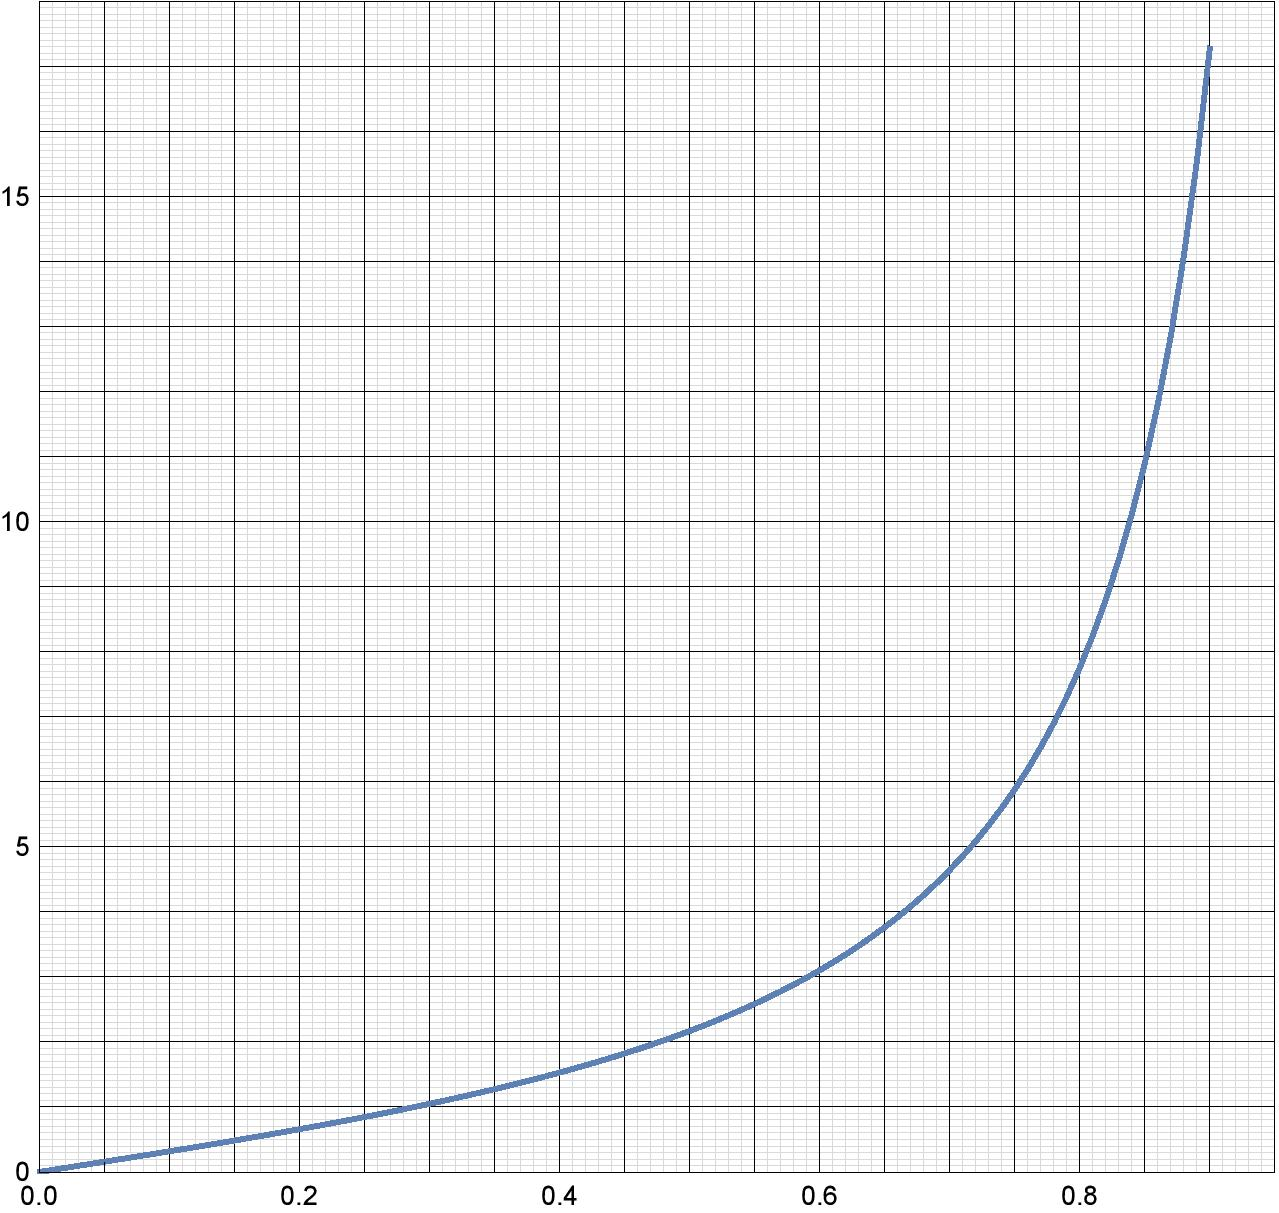
\includegraphics[width=0.72\textwidth]{T6_EN_assets/fig4.jpg}
    \caption{Figure 4.}
\end{figure}

\problembox{C4}{For the semi-infinite cylinder under consideration, find the magnitude of the electric field strength at point $A$, located at a distance $r=0.9R$ from point $O$.}{3.00}

\vspace{1em}
\noindent\textit{Source:} \url{https://pho.rs/p/66}

\end{document}